\section{Pressure}

%Concept of Pressure

\subsection{Balloon Pop}
\begin{itemize}
\item{Preparation Time: 20 minutes}
\item{Materials: piece of wood, nails, water balloons, water}
\item{Procedure: Put one nail through the board in one place and a large cluster of closely spaced nails in another place, all pointing up. Fill a balloon with water. As you lower the balloon onto the single or few nails, the balloon eventually pops. Fill another balloon with water and slowly lower it onto the cluster of nails. It should not pop.}
\item{Theory: As area of a force increases, pressure decreases. Therefore, as more nails are added and the area of the force (the weight of the balloon) increases, the pressure decreases and the balloon does not pop. Or, it takes more force to pop.}
\item{Alternative: hang the balloon from a spring balance as you lower it (by holding the spring balance) onto the nails. The difference in weight will allow you to calculate the force needed to pop the balloon.}
\end{itemize}

\subsection{Potato Poke}
\begin{itemize}
\item{Preparation Time: none}
\item{Materials: some straws, potato}
\item{Procedure: Take a straw and jab it into the potato. The straw should bend easily leaving the potato unharmed. Now place your thumb firmly over one end of a straw and jab the other end into the potato. This time the straw should enter the potato quite easily.}
\item{Theory: The straw is weaker than the potato and so will bend rather than break the potato’s skin. But, with your thumb plugging the back of the straw, the air inside the straw cannot leave and instead pushes out against the sides of the straw. As the straw strikes the potato, it cannot bend with the air pressure inside and so instead can poke through the skin into the potato.}
\end{itemize}


%\subsection{Air Pressure}
%
%\subsubsection*{Learning Objectives}
%\begin{itemize}
%\item{To observe the effects of air pressure on a flexible material}
%\end{itemize}
%
%\subsubsection*{Background Information}
%Air in a container pushes out with equal force on all sides of the container. If the pressure in the container is low, the force is small; if the pressure is high, the force is large. If the pressure is high, it is difficult to bend or crush the container as the air pressure inside resists being pushed. If the pressure is high enough, it can cause a flexible container to be rigid.
%
%\subsubsection*{Materials}
%Plastic straw, potato
%
%\subsubsection*{Activity Procedure}
%\begin{enumerate}
%\item{Hold a straw and push it hard into the potato.}
%\item{Observe what happens to the straw.}
%\item{Place your thumb firmly over one end of a straw and push the other end into the potato.}
%\item{Observe what happens to the straw and potato.}
%\end{enumerate}
%
%\subsubsection*{Cleanup Procedure}
%Dispose of the potato and return the straw to its proper place.
%
%\subsubsection*{Discussion Questions}
%\begin{enumerate}
%\item{Why does the straw not pierce the potato when your thumb is not blocking the back of the straw?}
%\item{Why does the straw pierce the potato when your thumb is blocking the potato?}
%\end{enumerate}
%
%\subsubsection*{Results and Conclusions}
%When the straw is pushed into the potato, it bends. The skin of the potato is strong enough that the straw cannot pass through it. However, when your thumb covers the back of the straw, the straw breaks the skin of the potato and passes through. This is because the air in the straw pushes out against the sides of the straw. Without your thumb, the air can simply escape out the back of the straw without applying a force. When your thumb covers the hole, the air cannot go anywhere so it applies a force outward. This causes the side of the straw to become rigid, allowing it to break the skin of the potato.
%
%\subsubsection*{Notes}
%Be sure that, in the first step, you are not holding your thumb over the back of the straw. This should only be done later.

%Pressure Due to Solids

\subsection{The Effect of Surface Area on Pressure}

\subsubsection*{Learning Objectives}
\begin{itemize}
\item{To observe the factors affecting pressure} 
\item{To demonstrate the effects of surface area on pressure} 
\end{itemize}

\subsubsection*{Background Information}
When a force acts on an object, the results are greatly affected by the area over which it acts. Consider the pain in your hand when you carry a bucket of water with a thin wire handle. Wrapping a piece of fabric around the handle greatly reduces the pain. This can be explained using pressure and summarized in the equation:
$$\mathrm{Pressure} = \mathrm{Force} \times \mathrm{Area}$$
$$P=F\times A$$

\subsubsection*{Materials}
Bar of soap, thin thread, thick string, 4 heavy stones of approximately equal weight, two stools, and a small wooden board.

\subsubsection*{Activity Procedure}
\begin{enumerate}
\item{Place the wooden board between the two stools.}
\item{Place the piece of soap on top of the wooden board. }
\item{Tie stones to the ends of the thick string. Then tie stones to the end of the thin thread.} 
\item{Hang each type of thread across the bar of soap so that the stones hang freely.} 
\item{Observe the effect of each thread on the bar of soap.} 
\end{enumerate}

\begin{figure}
\begin{center}
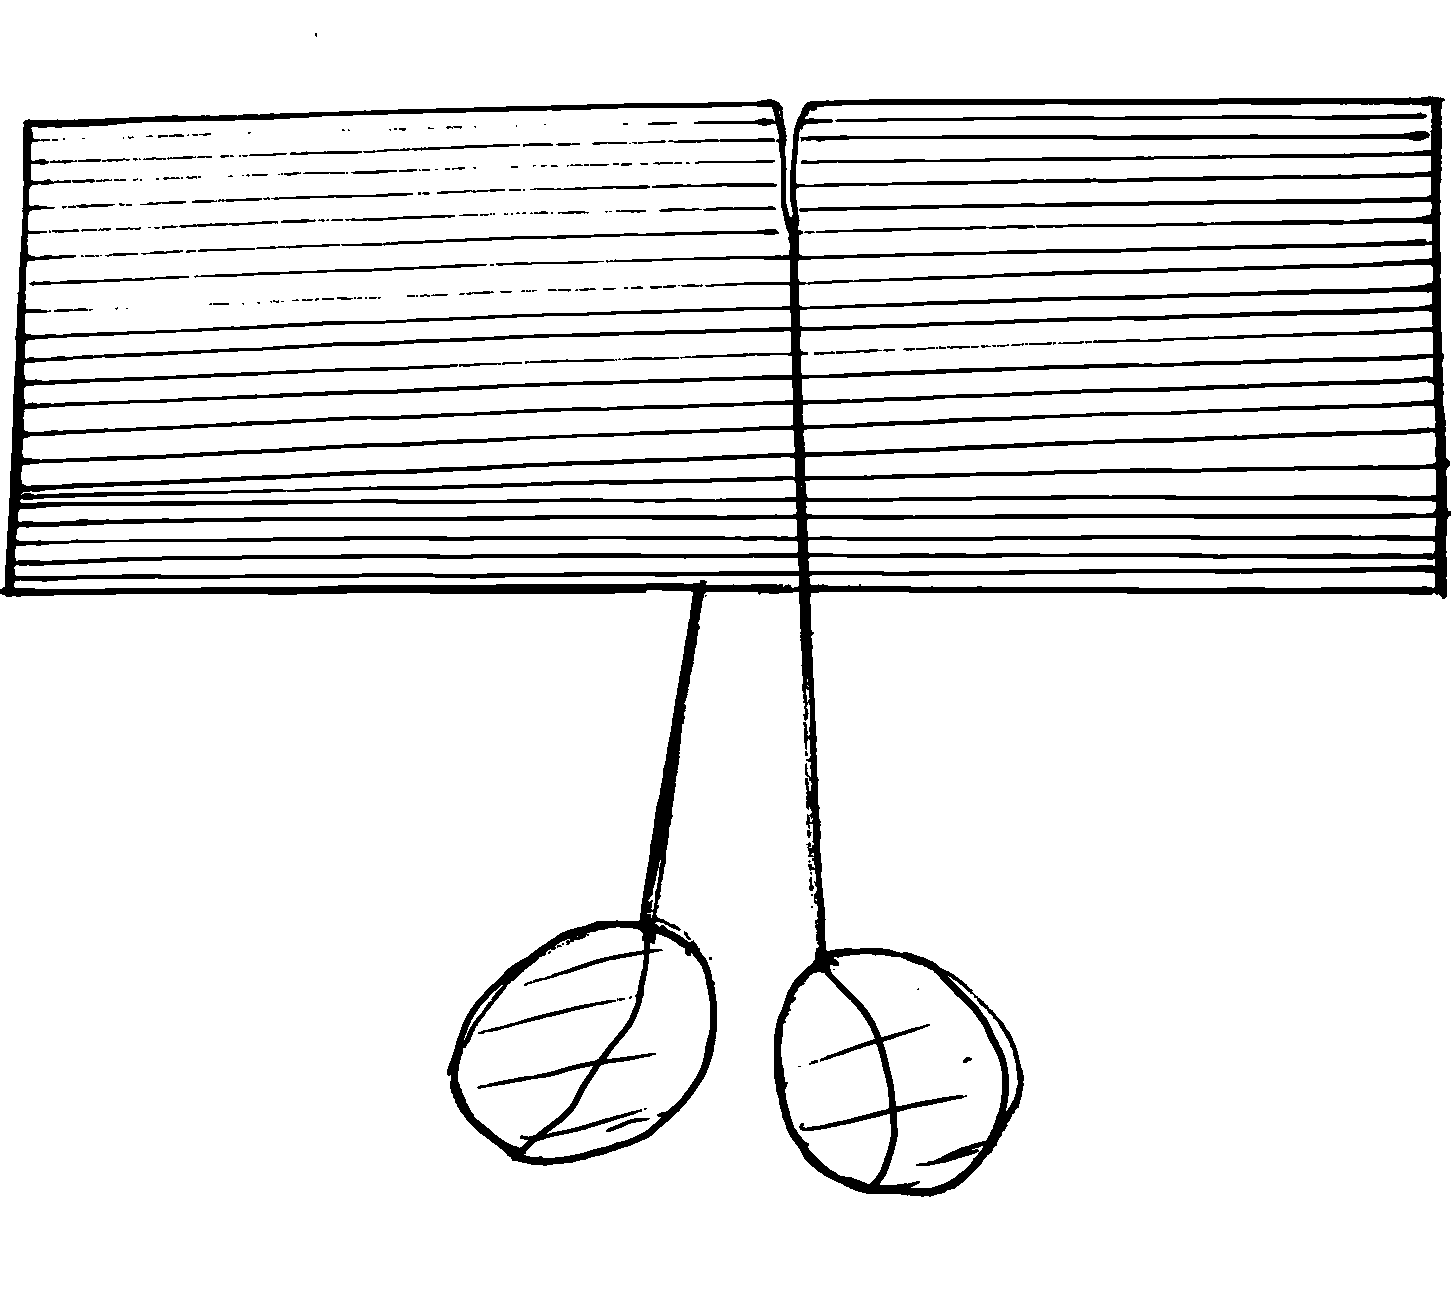
\includegraphics{./img/pressure-solid1.png}
\caption{Thin Thread}
\label{fig:pressure-solid1}
\end{center}
\end{figure}

\begin{figure}
\begin{center}
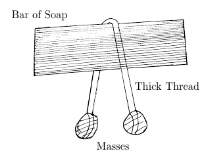
\includegraphics{./img/pressure-solid2.png}
\caption{Thick String}
\label{fig:pressure-solid2}
\end{center}
\end{figure}

\subsubsection*{Results and Conclusions}
It will be seen that the bar of soap was cut easily by using a thin thread but not by using a thick string. This because the thin thread has a small surface area and the same force and therefore a large pressure, while the thick thread has a larger area for the same force and therefore smaller pressure. 

\subsubsection*{Clean Up Procedure}
Collect all the used materials, cleaning and storing items that will be used later.

\subsubsection*{Discussion Question}
Why does a thin thread cut easily through a bar of soap while a thick thread does not?


%Pressure in Liquids


\subsection{Straw Fountain}
\begin{itemize}
\item{Preparation Time: 10 minutes}
\item{Materials: 0.5 liter water bottle with cap, water, straw, glue}
\item{Procedure: Poke a hole with the diameter of the straw in the cap of the water bottle with a hot nail or pin. Insert the straw so that it extends almost to the bottom of the water bottle and leaves enough sticking out for your mouth. Secure it with glue so that it is airtight. When the glue is dry, fill the bottle about half way with water and close the cap with the straw inside. Have a student blow as hard as they can through the straw into the water. When they run out of air and stop blowing, they will get a nice spray in the face. }
\item{Theory: By blowing into the bottle, you greatly increase the pressure inside. When you finish blowing, the pressure will try to equilibrate by forcing the pressure back out through the straw. There is nowhere for the water to go but out.}
\end{itemize}


\subsection{Cartesian Diver}

\subsubsection*{Learning Objectives}
\begin{itemize}
\item{To observe characteristics of a submerging body}
\item{To describe and apply the concept of Cartesian diver in daily life}
\end{itemize}

\subsubsection*{Background Information}
When the body is immersed in a liquid it may sink or float. The body will float in water when its density is less than density of water. A submerging body is designed in such a way that it will sink a little but also float in water. 

\subsubsection*{Materials}
Large Bottle (1.5 litres) or transparent long container with a cover or cap, water, syringe, and small stones

\subsubsection*{Preparation Procedure}
Remove the needle from the syringe.

\subsubsection*{Activity Procedure}
\begin{enumerate}
\item{Fill a bottle with some water.}
\item{Remove the plunger from the syringe and insert a few stones into the syringe.}
\item{Replace the plunger so that the syringe is full of air but sealed at the top.} 
\item{Hold the syringe upright and immerse it in the bottle making sure that the syringe and its contents float upright in the water.}
\item{Close the bottle with the cap.}
\item{Gently squeeze the bottle near the bottom.} 
\item{Observe what happens.}
\end{enumerate}

\begin{figure}
\begin{center}
\def\svgwidth{100pt}
\input{./img/cartesian-diver.pdf_tex}
\caption{The Cartesian Diver}
\label{fig:cartesian-diver}
\end{center}
\end{figure}

\subsubsection*{Results and Conclusions}
When the bottle is gently squeezed the syringe sinks down to the bottom. When the bottle is released the syringe rises back up. 

\subsubsection*{Discussion Question}
Why does the syringe move down when the bottle is squeezed?

\subsubsection*{Notes}
The syringe sinks down because the pressure in the bottle increases when you squeeze it. Added pressure will cause water from the bottle to enter into the syringe through the needle hole. This increases the weight of the syringe and thus it sinks. When the pressure is released, the water in the syringe leaves and so the syringe will float again. A Cartesian diver and a submarine use the same principle to sink and float in deep water.

	%Variation of Pressure with Depth
	
\subsection{Holey Bottle 2}
\begin{itemize}
\item{Preparation Time: 10 minutes}
\item{Materials: Water bottle, pin or small nail, water, bucket (for catching water)}
\item{Procedure: In even intervals around the base of the water bottle, poke small holes with the pin or nail. Try to get an even distribution and the same size hole all around. Fill the bottle with water and watch the water leave each hole with the same force. Blowing into the bottle will help illustrate the equality of the pressure in all directions.}
\item{Theory: Pressure in a fluid acts equally in all directions, therefore the water being forced out the bottom should feel the same amount of pressure and shoot the same distance.}
\end{itemize}


%\subsection{Holey Bottle 1}
%\begin{itemize}
%\item{Preparation time: 5 minutes}
%\item{Materials: empty 1.5 liter water bottle, water}
%\item{Construction: Pierce three or more small (less than 0.5cm) neat holes in the water bottle, at different vertical heights. An easy way to do this is to use firm but gently pressure with a metal needle from a syringe. Make sure to pierce the bottle in parts that are vertical, not parts that slope in or out.}
%\item{Procedure: Fill the bottle with water and place it on the ground or on a table. Water will pour out of the bottle through the small holes. Note that the streams of water strike the ground at different distances from the bottle. At any given time, the hole that is closest to one-half of the height of the water level should strike the ground or table at the greatest distance from the bottle.}
%\item{Theory: To understand this we must consider both Bernoulli’s Principle and Projectile Motion. Bernoulli’s Principle tells us that the horizontal speed of each stream of water varies as the square root of the depth from the surface of the water. Projectile Motion tells us that the distance reached by a stream of water is proportional to the velocity of the water and to the time before the water strikes the ground. The time before the water strikes the ground is proportional to the square root of the height above the ground. Combining these two factors, we find that the maximum distance will be reached for a stream of water that is halfway between the ground and the surface.}
%\end{itemize}


\subsection{Liquid Pressure and Depth}

\subsubsection*{Learning Objectives}
\begin{itemize}
\item{To verify the variation of pressure with depth in water} 
\end{itemize}

\subsubsection*{Background Information}
The wall of a dam is made much thicker at the bottom than at the top. Also, water storage tanks are placed at the top of a building. This is because the pressure in a liquid is related to its depth.

\subsubsection*{Materials}
Plastic bottle, nail or metal pin/needle, matches, water


\subsubsection*{Preparation Procedure}
\begin{enumerate}
\item{Light a match and heat the sharp point of the nail or pin.} 
\item{Use the heated nail to put three holes into a bottle. Put one hole near the bottom, one near the middle, and the last hole between them.} 
\end{enumerate}

\subsubsection*{Activity Procedure}
\begin{enumerate}
\item{Fill the bottle with water up to the rim.} 
\item{Hold the bottle in air using your hand or place the bottle at the top of a tall object like a stool on a table.} 
\item{Allow water to flow out of the bottle and observe the trajectory of water from each hole. Note the horizontal distance reached of water from each hole.} 
\end{enumerate}

\begin{figure}
\begin{center}
%\def\svgwidth{200pt}
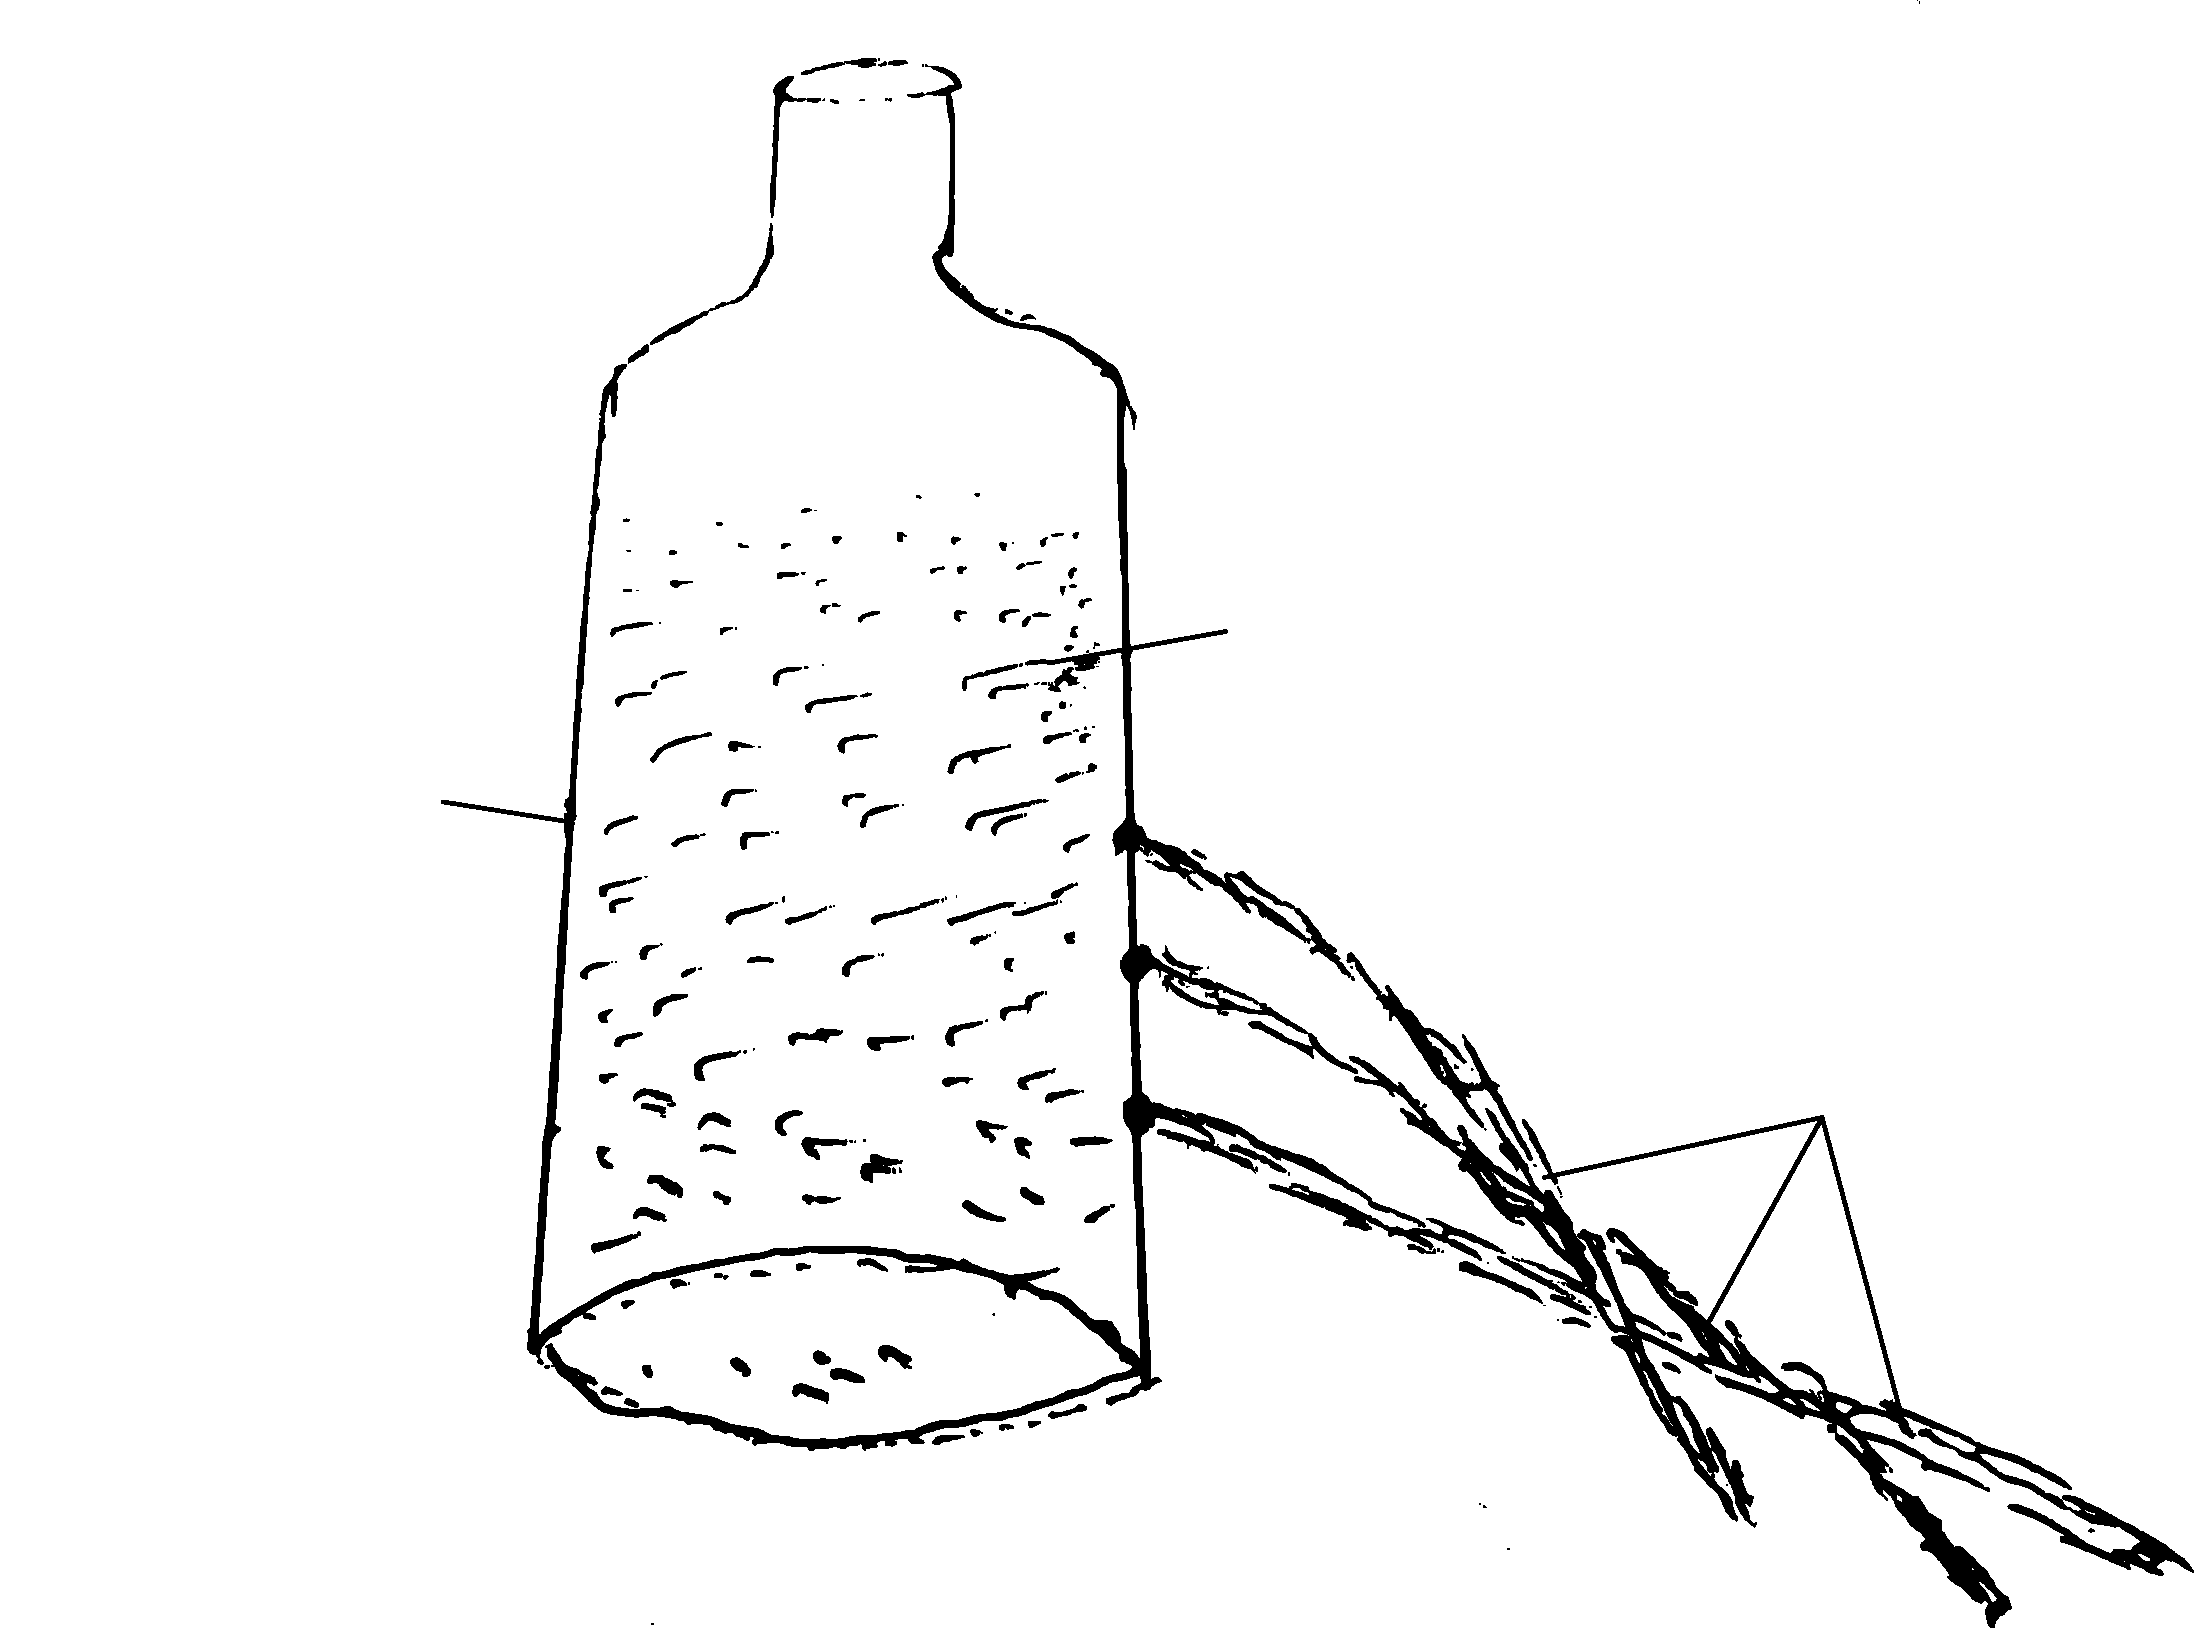
\includegraphics{./img/pressure-liquid.png}
\caption{Demonstration of the effect of depth on liquid pressure}
\label{fig:pressure-liquid}
\end{center}
\end{figure}

\subsubsection*{Results and Conclusions}
The water flows faster from the hole with the greater depth because there is greater pressure, showing that the water pressure increases with the depth of the water. This is because the weight of the water on top acts downward causing pressure. The greater the depth, the greater the weight, resulting in greater pressure. 

\subsubsection*{Clean Up Procedure}
Collect all the used materials, cleaning and storing items that will be used later.

\subsubsection*{Discussion Questions}
\begin{enumerate}
\item{What have you observed in the trajectory of water from each hole?}
\item{How does the pressure change with the depth of water? Why?}
\end{enumerate}

\subsubsection*{Notes}
There is a difference between depth and height. Height is measured from the reference point upward while depth is measured from the reference point downward. The reference point in this case is at the surface of water. 
%The holes must not be in the same vertical line in order to view the flow clearly. 	
	

	%Hydraulic Press
	
\subsection{Hydraulic Press}
\begin{itemize}
\item{Preparation Time: 15 minutes}
\item{Materials: Two syringes of different sizes (50 ml and 20 ml work well), thin rubber tubing, water}
\item{Procedure: Fill the larger syringe with water and attach one end of the rubber tubing to its end. Attach the other end of the tubing to the smaller syringe (the plunger should be inserted all the way in the smaller syringe). Pushing the plunger of the larger syringe will cause the plunger of the smaller syringe to go out, and vice-versa. You will notice that it is easier to push the plunger of the small syringe than that of the larger syringe.}
\item{Theory: Pressure is equal to force per area, and the pressure is distributed equally throughout a liquid. As such, the pressure at one plunger must be equal to the pressure at the other plunger. Setting the two ratios equal, we can see that a small force over a small area can overcome a large force over a large area.}
\end{itemize}

\begin{figure}[h!]
\begin{center}
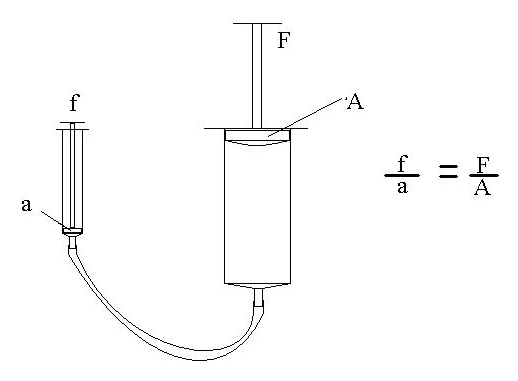
\includegraphics{./img/hydraulic-press.png}
\caption{A hydraulic press}
\label{fig:hydraulic-press}
\end{center}
\end{figure}
	

	%Manometer
	
%Atmospheric Pressure [See Gas Laws in Chem - Charles' Law]


\subsection{Atmospheric Pressure}
\begin{itemize}
\item{Preparation Time: 5 minutes}
\item{Materials: Water bottle, pin and/or nail, water}
\item{Procedure: Using an empty water bottle (bigger is better), poke four or five small holes (0.5 cm) in the bottom with the pin and then the nail. Fill the bottle about half way with water, allowing it to spill out through the holes in the bottom. While the students are watching, seal the cap on the bottle. The water will cease to pour out of the bottom despite the holes and rather predictable effect of gravity. When the gasps of wonder die down, discuss the following:}
\item{Theory: The pressure of the water combined with the pull of gravity is enough to cause the water to pour through the holes in the bottle when the cap is not sealed. When the cap is on tight, however, the combined high air pressure outside the bottle and low air pressure inside the bottle creates enough of an upward force on the water to counter the downward force of gravity.}
\end{itemize}


\subsection{Charles' Law, Part C -- Bottle Crush}
\begin{itemize}
\item{Preparation time: 10 minutes}
\item{Materials: water bottle, boiling water}
\item{Procedure: pour some boiling water into the water bottle. Cap the bottle and shake to make sure all the air in the bottle is heated from the hot water. Open the bottle and pour out the liquid. Recap the bottle. After a short time, the bottle will contract.}
\item{Theory: Charles' law states that volume is proportional to temperature. By capping the hot air inside of the water bottle, the volume of the air inside the bottle will decrease as the temperature of the gas cools off. As the volume of the air reduces, the atmospheric pressure crushes the plastic water bottle.}
\end{itemize}


\subsection{Straw Elevator}
\begin{itemize}
\item{Preparation Time: none}
\item{Materials: two straws, container, water}
\item{Procedure: Fill the container with water and insert one straw so that it stands vertically in the water. Using the other straw, blow across the opening of the vertical straw; the water level in the straw will rise.}
\item{Theory: Bernoulli’s Principle states that moving air causes low pressure; the air passing in a stream over the vertical straw creates low pressure and therefore a pressure differential between the bottom of the straw (the water) and the top. The water will move towards the lower pressure, moving up the straw.}
\end{itemize}


\subsection{Making a Magdeburg Hemisphere}

\subsubsection*{Learning Objectives}
\begin{itemize}
\item{To demonstrate the effect of atmospheric pressure} 
\end{itemize}

\subsubsection*{Materials}
Two small cooking pots of equal size, oil, matches, small pieces of paper

\subsubsection*{Preparation Procedure}
Spread oil or grease around the edge of one of the cooking pots.

\subsubsection*{Activity Procedure}
\begin{enumerate}
\item{Place some pieces of paper into the cooking pot which does not have any oil.} 
\item{Light the pieces of paper on fire.} 
\item{Allow the paper to burn until about half of it has burned.} 
\item{Place the greased cooking pot upside-down on top of the ungreased cooking pot so that they create a sort of ball and no air can escape.} 
\item{Allow the pots to cool.} 
\item{Try to separate the pots.} 
\end{enumerate}

\subsubsection*{Results and Conclusions}
After the pots have cooled it is very difficult to separate them. This is because when you burn the paper, the air in the pot expands and escapes. When you cover the pots, no more air can enter and the air inside cools, reducing the pressure inside the pots while the pressure outside the pots remains the same. The atmospheric pressure therefore presses the pots together so as to equalize the pressure on either side of the pot. 



\subsubsection*{Clean Up Procedure}
Collect all the used materials, cleaning and storing items that will be used later.

\subsubsection*{Discussion Questions}
\begin{enumerate}
\item{What is the reason for burning the paper and then covering the pot?}
\item{What happens when the pots cool?}
\end{enumerate}

\subsubsection*{Notes}
The principle behind the Magdeburg hemisphere is used to create suction. When air is heated, it expands and escapes. If the hot container is sealed and allowed to cool, the reduced number of particles causes a lower pressure than atmospherric pressure. Thus, the force pushing the two pots together from the outside is greater than the force pushing out from the inside and thus the two pots are very difficult to separate. 

	%Barometer
	
	%Siphon
	
\subsection{Siphon}
\begin{itemize}
\item{Preparation Time: 1 minute}
\item{Materials: two containers, half meter of rubber tubing/IV line/feeding tube, water}
\item{Procedure: Place one jar with water on a table and the other empty jar on a chair just below the table. Place one end of the tubing into the water and the other in your mouth. Suck on the tube until the water starts coming out and place the end of the tube into the empty beaker, holding the middle of the tube at the level of your mouth. The water will continue to flow from the water jar to the empty jar, despite the water’s initial uphill climb.}
\item{Theory: By sucking on the tubing, you create low pressure on that side. The slightly higher pressure (atmospheric) at the water will cause the water to continue to travel as long as the pressure difference is enough to overcome gravity. If you raise the middle of the tube too high, the water will stop flowing.}
\end{itemize}


%\subsection{A Siphon}
%
%\subsubsection*{Learning Objectives}
%\begin{itemize}
%\item{To demonstrate how to shift water from one bucket to another bucket using suction} 
%\item{To identify the applications of atmospheric pressure} 
%\end{itemize}
%
%\subsubsection*{Materials}
%Two buckets, water, thick rubber tube about 1 m long
%
%\subsubsection*{Activity Procedure}
%\begin{enumerate}
%\item{Pour some water into a bucket and place it on the table. Place the other bucket below the table.} 
%\item{Put the rubber tube in the bucket and fill it with water.} 
%\item{Bend one end of the tube so that air cannot enter and remove it from the bucket. Make sure the other end of the tube remains underwater.}
%\item{Lower the bent end of the tube into the lower bucket.}
%\item{Open the bent end. Observe what happens.} 
%\end{enumerate}
%
%\subsubsection*{Results and Conclusions}
%Water will flow from the bucket on the table to the other bucket below the table. This is because of the combined force of atmospheric pressure pushing in the top bucket and gravity pulling the water to the bottom bucket.
%
%\subsubsection*{Clean Up Procedure}
%Collect all the used materials, cleaning and storing items that will be used later.
%
%\subsubsection*{Discussion Question}
%If the two buckets were switched, would the water flow from the lower bucket to a bucket on the table? Explain your answer.
%
%\subsubsection*{Notes}
%The flow of water is driven by the net difference in elevation of the two ends of the tube. The force of gravity pulls the water through a siphon. As long as the inlet is above the outlet, water will flow even if it has to go up before it goes down. This is because as water is pulled down the of the tube by gravity the pressure decreases at the top of the siphon and air pressure in the bucket pushes the water into the tube. This will continue until the water level in the top bucket is below the inlet of the tube.	
	

\subsection{Automatic Flushing Tank}

\subsubsection*{Learning Objectives}
\begin{itemize}
\item{To identify the application of pressure differences}
\end{itemize}

\subsubsection*{Background Information}
The effect of pressure in a liquid can be observed in different ways. Automatic flushing tanks operate under the influence of pressure in a liquid. When the level of water in a container reaches the highest point in the exit pipe, water will drain from the tank until the level of the water in the tank is below the level of the outlet. The tank can then be refilled to repeat the cycle. This type of system is useful for flushing or when you need a certain amount of water for a given amount of time.

\subsubsection*{Materials}
Empty drinking water bottle, straw, water, bucket, chewing gum OR superglue

\begin{figure}
\begin{center}
\def\svgwidth{100pt}
\input{./img/auto-flushing-tank.pdf_tex}
\caption{The Automatic Flushing Tank}
\label{fig:auto-flushing-tank}
\end{center}
\end{figure}

\subsubsection*{Preparation Procedure}
Cut off the top of an empty water bottle, make a hole at the bottom so as to fit the straw through it. 
Bend the straw inside the bottle so that it makes an upside down 'U' shape. Use the chewing gum or superglue to seal the hole.

\subsubsection*{Activity Procedure}
\begin{enumerate}
\item{Hold the bottle and place the bucket below the bottle.} 
\item{Pour some water into the bottle up to and above the bend in the straw and observe what happens.} 
\end{enumerate}

\subsubsection*{Results and Conclusions}
The water will flow into the bucket through the bent straw. 

\subsubsection*{Clean Up Procedure}
Collect all the used materials, cleaning and storing items that will be used later.

\subsubsection*{Discussion Question}
What causes the water to flow from the bottle to the bucket? How does this work?

\subsubsection*{Notes}
The siphon principle states that liquid is able to flow without pumping because the combined pressure of the water and the atmosphere pushing down on the water is greater then the air pushing up on the straw. The automatic flushing tank does not require a handle to trigger the flush. Once the water flows into the tank up to the level of the siphon, the tank will flush automatically. 
	
	
	
	%Pumps (Lift Pump, Force Pump, Bicycle Pump)


\subsection{Reverse Air Pump}
\begin{itemize}
\item{Preparation Time: varies, about 1 hour}
\item{Materials: Bicycle pump (the tall, metal kind), short piece of rubber tubing fitted to pump valves, utility knife, tightening sleeves, extra valve}
\item{Procedure: There are two parts of the pump that control the direction of airflow: the first is a diaphragm inside the pump and the second is a ball valve at the base of the pump in the hose.
\begin{enumerate}
\item{You need to open the pump and pull out the ‘dipstick’ with the diaphragm attached. At the bottom, there should be a diaphragm with holes around the top, a metal disc the same diameter as the diaphragm, and a few nuts and washers to keep it all together. In its normal configuration, the diaphragm is pulled down by friction away from the disc when the pump handle is pulled up, allowing air to enter the pump freely. When the pump handle is pushed in, the diaphragm is forced against the disc, restricting any back airflow, and forcing all the air forward through the hose. Switch the position and direction of the diaphragm and disc so that it has the opposite effect when the pump handle is pulled in or out.}
\item{Next, you need to cut open the hose at the base of the pump and find the valve with the small bead inside. Normally, when air is forced forward through the valve, the bead does not restrict any airflow. When air tries to go back through the pump, the bead blocks the valve and stops any airflow. Switch the direction of the valve.}
\item{From here, you need to reattach the hose to the pump. You may need to get another nozzle to attach to the pump, attaching the hose with reversed valve with the extra bit of rubber tubing. It depends on your pump, but if you have made it this far, you will find a way to make it work. Tightening sleeves will come in handy here to make sure no air is lost after all this cutting and jury-rigging.}
\end{enumerate}
} % Procedure
\item{Applications: This suction pump is great for showing the gas laws and boiling points: suck the air out of a jar of water and watch the water boil, you could also kill stuff in the jar this way, but that is just morbid, and possibly cool, or that sound travels through a medium.}
\end{itemize}
